\NewChapter{独木成林}

\quote{人类忘记了自己的起源,又无视维持生存最起码的需要,这样,水和其他资源也就一同变成了人类漠然不顾的受难者。}{《寂静的春天》}


《独木成林》是一款2D俯视角模拟经营类游戏。

森林已奄奄一息:自然条件恶劣,人类砍伐无度,只留下不屈的独木在大地上摇曳。所幸未到绝境,土地下还有着丰富的水源等待着根系的汲取,土地上倔强的树木还在为根系孜孜不倦地产出着有机物。

玩家将扮演绿洲之神,救森林于危难中。请利用好手中的水与有机物资源,向着大地的边界扩展你的根系,依靠着孤单的“初始之树”,建成葳蕤的森林。

WASD控制视角移动,鼠标点击交互进行地下视角与地面视角的切换,可在其中进行每回合最多两次的长根与长树操作。玩家初始拥有一定量的水与有机物,根耗有机物产水,树耗水产有机物,树只能长在根系覆盖的地块中。您的森林还将面临周期性的自然灾害,以及突发的人类砍伐行为的挑战。在30回合内,尽可能将森林发展壮大吧!

\section{创作历程}

游戏创作于2023年2月,为2023年Global Game Jam参赛作品,大赛主题为“Root”,团队三人于48小时之内完成设计开发。

由于Game Jam时间有限,我们团队进行了快速的头脑风暴并确定设计方向。我们在首先确定了类文明的六边形地图和策略游戏的主要基调,长树、长根并扩大绿化的游戏目标以及资源相互制约、步步为营的游戏体验目标。随后确定了游戏中只有两种资源:水和有机物。根系在地块中能获得水,树能产生有机物,玩家的长根和长树会消耗水和有机物。在此基础上拉表去确定具体数值,并在 Unity 内快速构建关卡编辑器根据体验设计关卡。

\begin{figure}[H]
\centering  %图片全局居中
\subfigure[线上头脑风暴]{
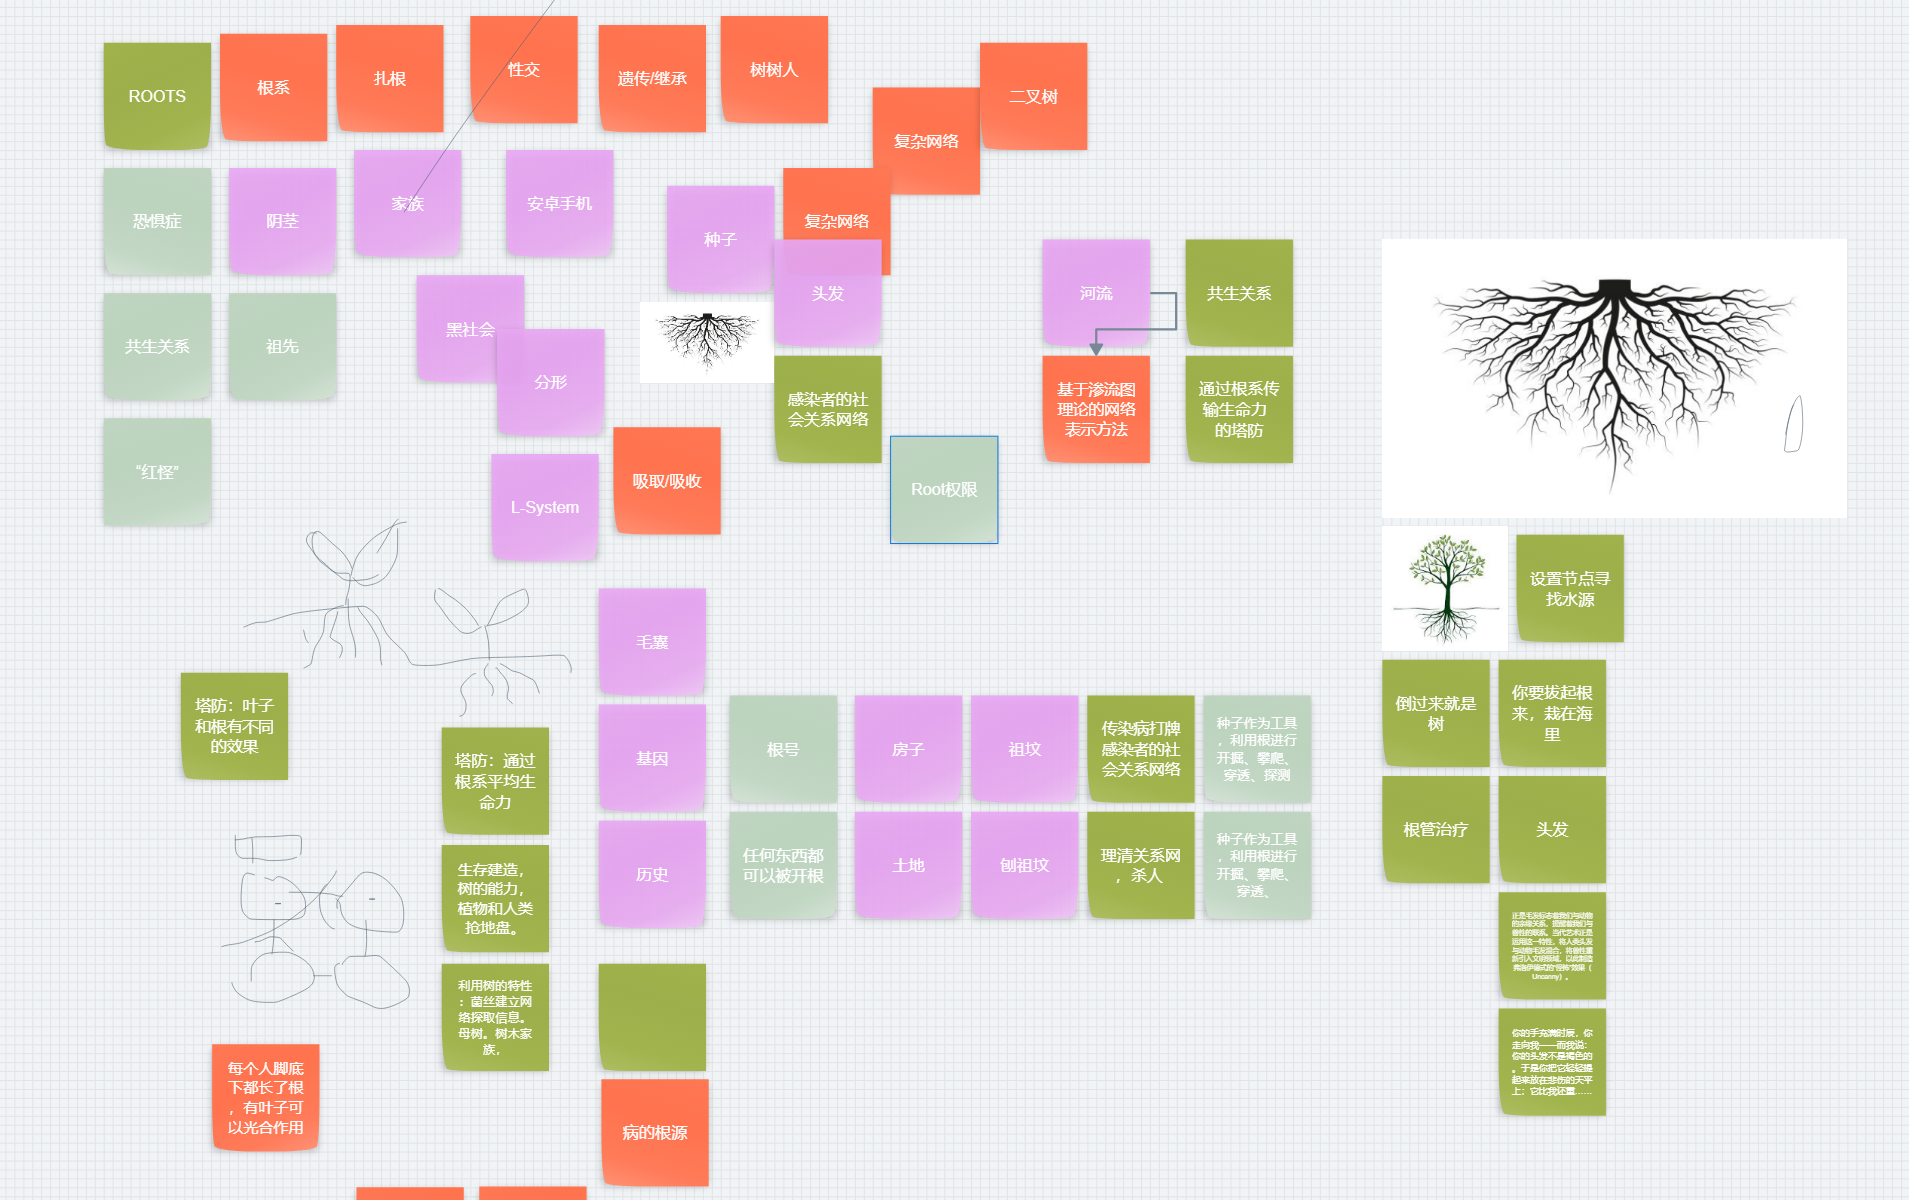
\includegraphics[width=0.45\textwidth]{Images/独木成林/ggj_brainstorm.png}}
\subfigure[电子纸面原型]{
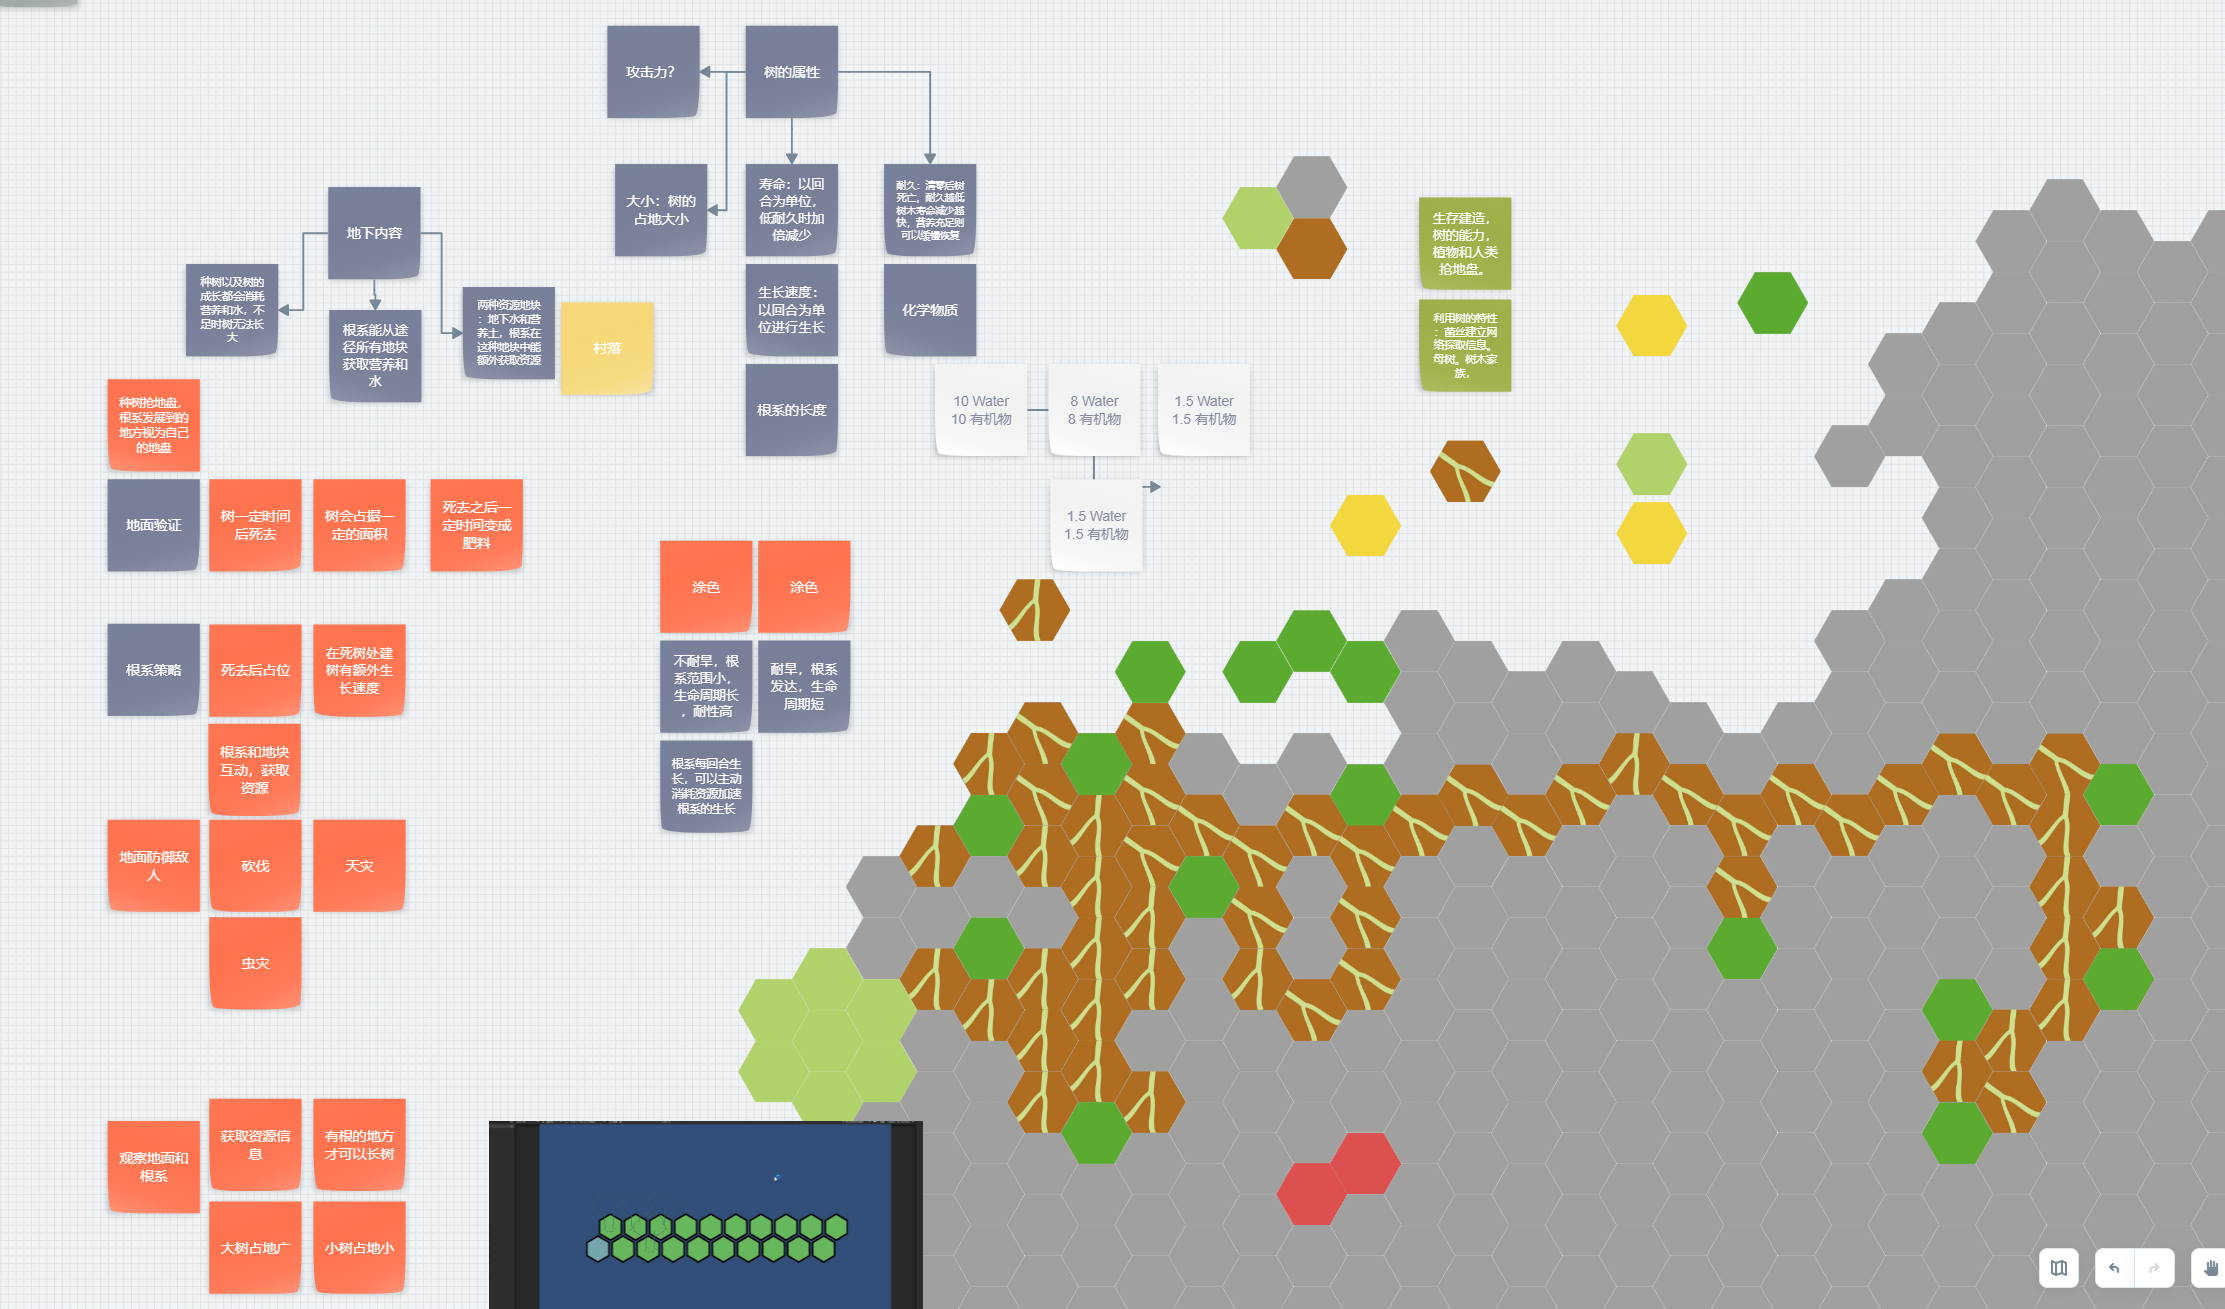
\includegraphics[width=0.45\textwidth]{Images/独木成林/ggj_design.png}}
\caption{原型设计环节}
\end{figure}

\begin{figure}[H]
    \centering
    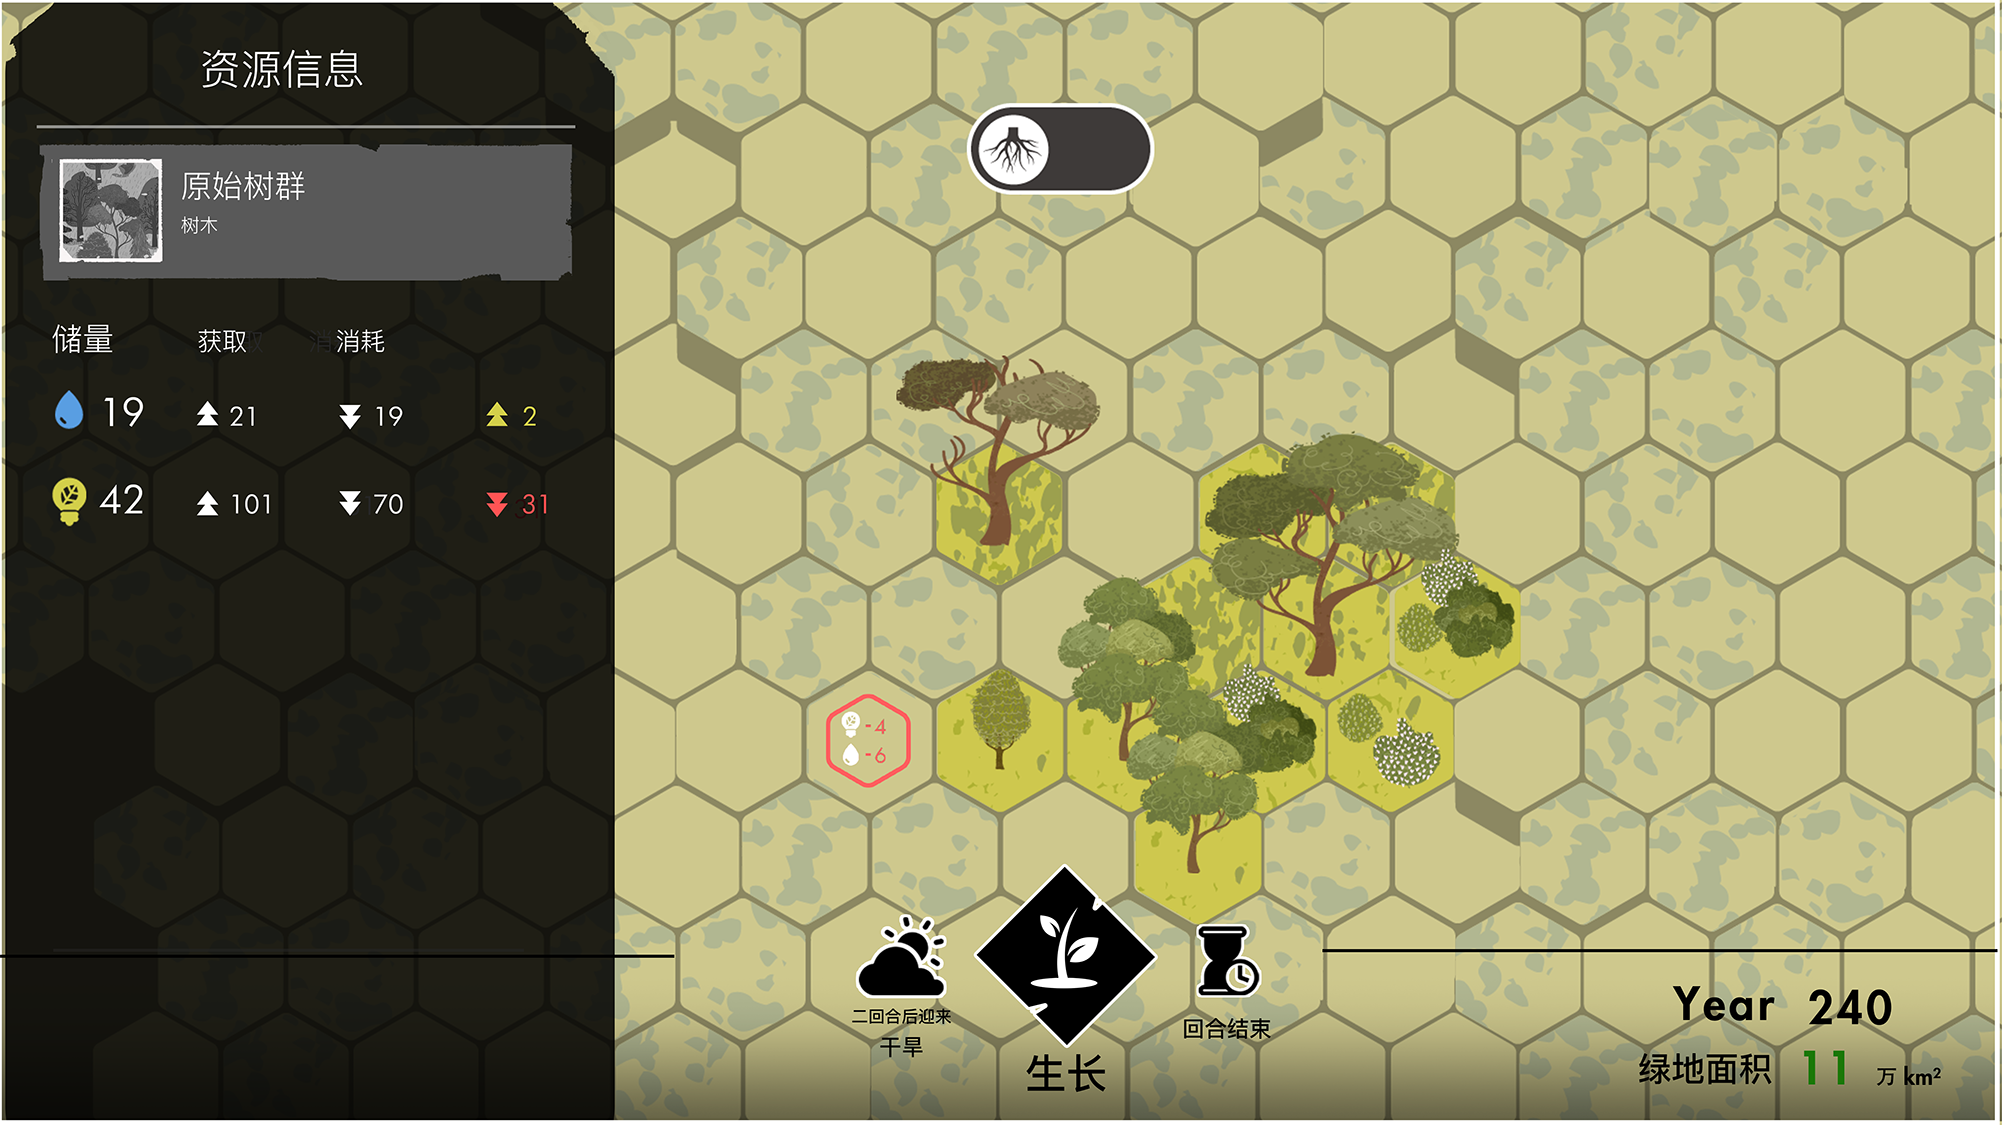
\includegraphics[width=0.8\textwidth]{Images/独木成林/dmzl1.png}
    \caption{独木成林\ 地上画面}
\end{figure}

\begin{figure}[H]
    \centering
    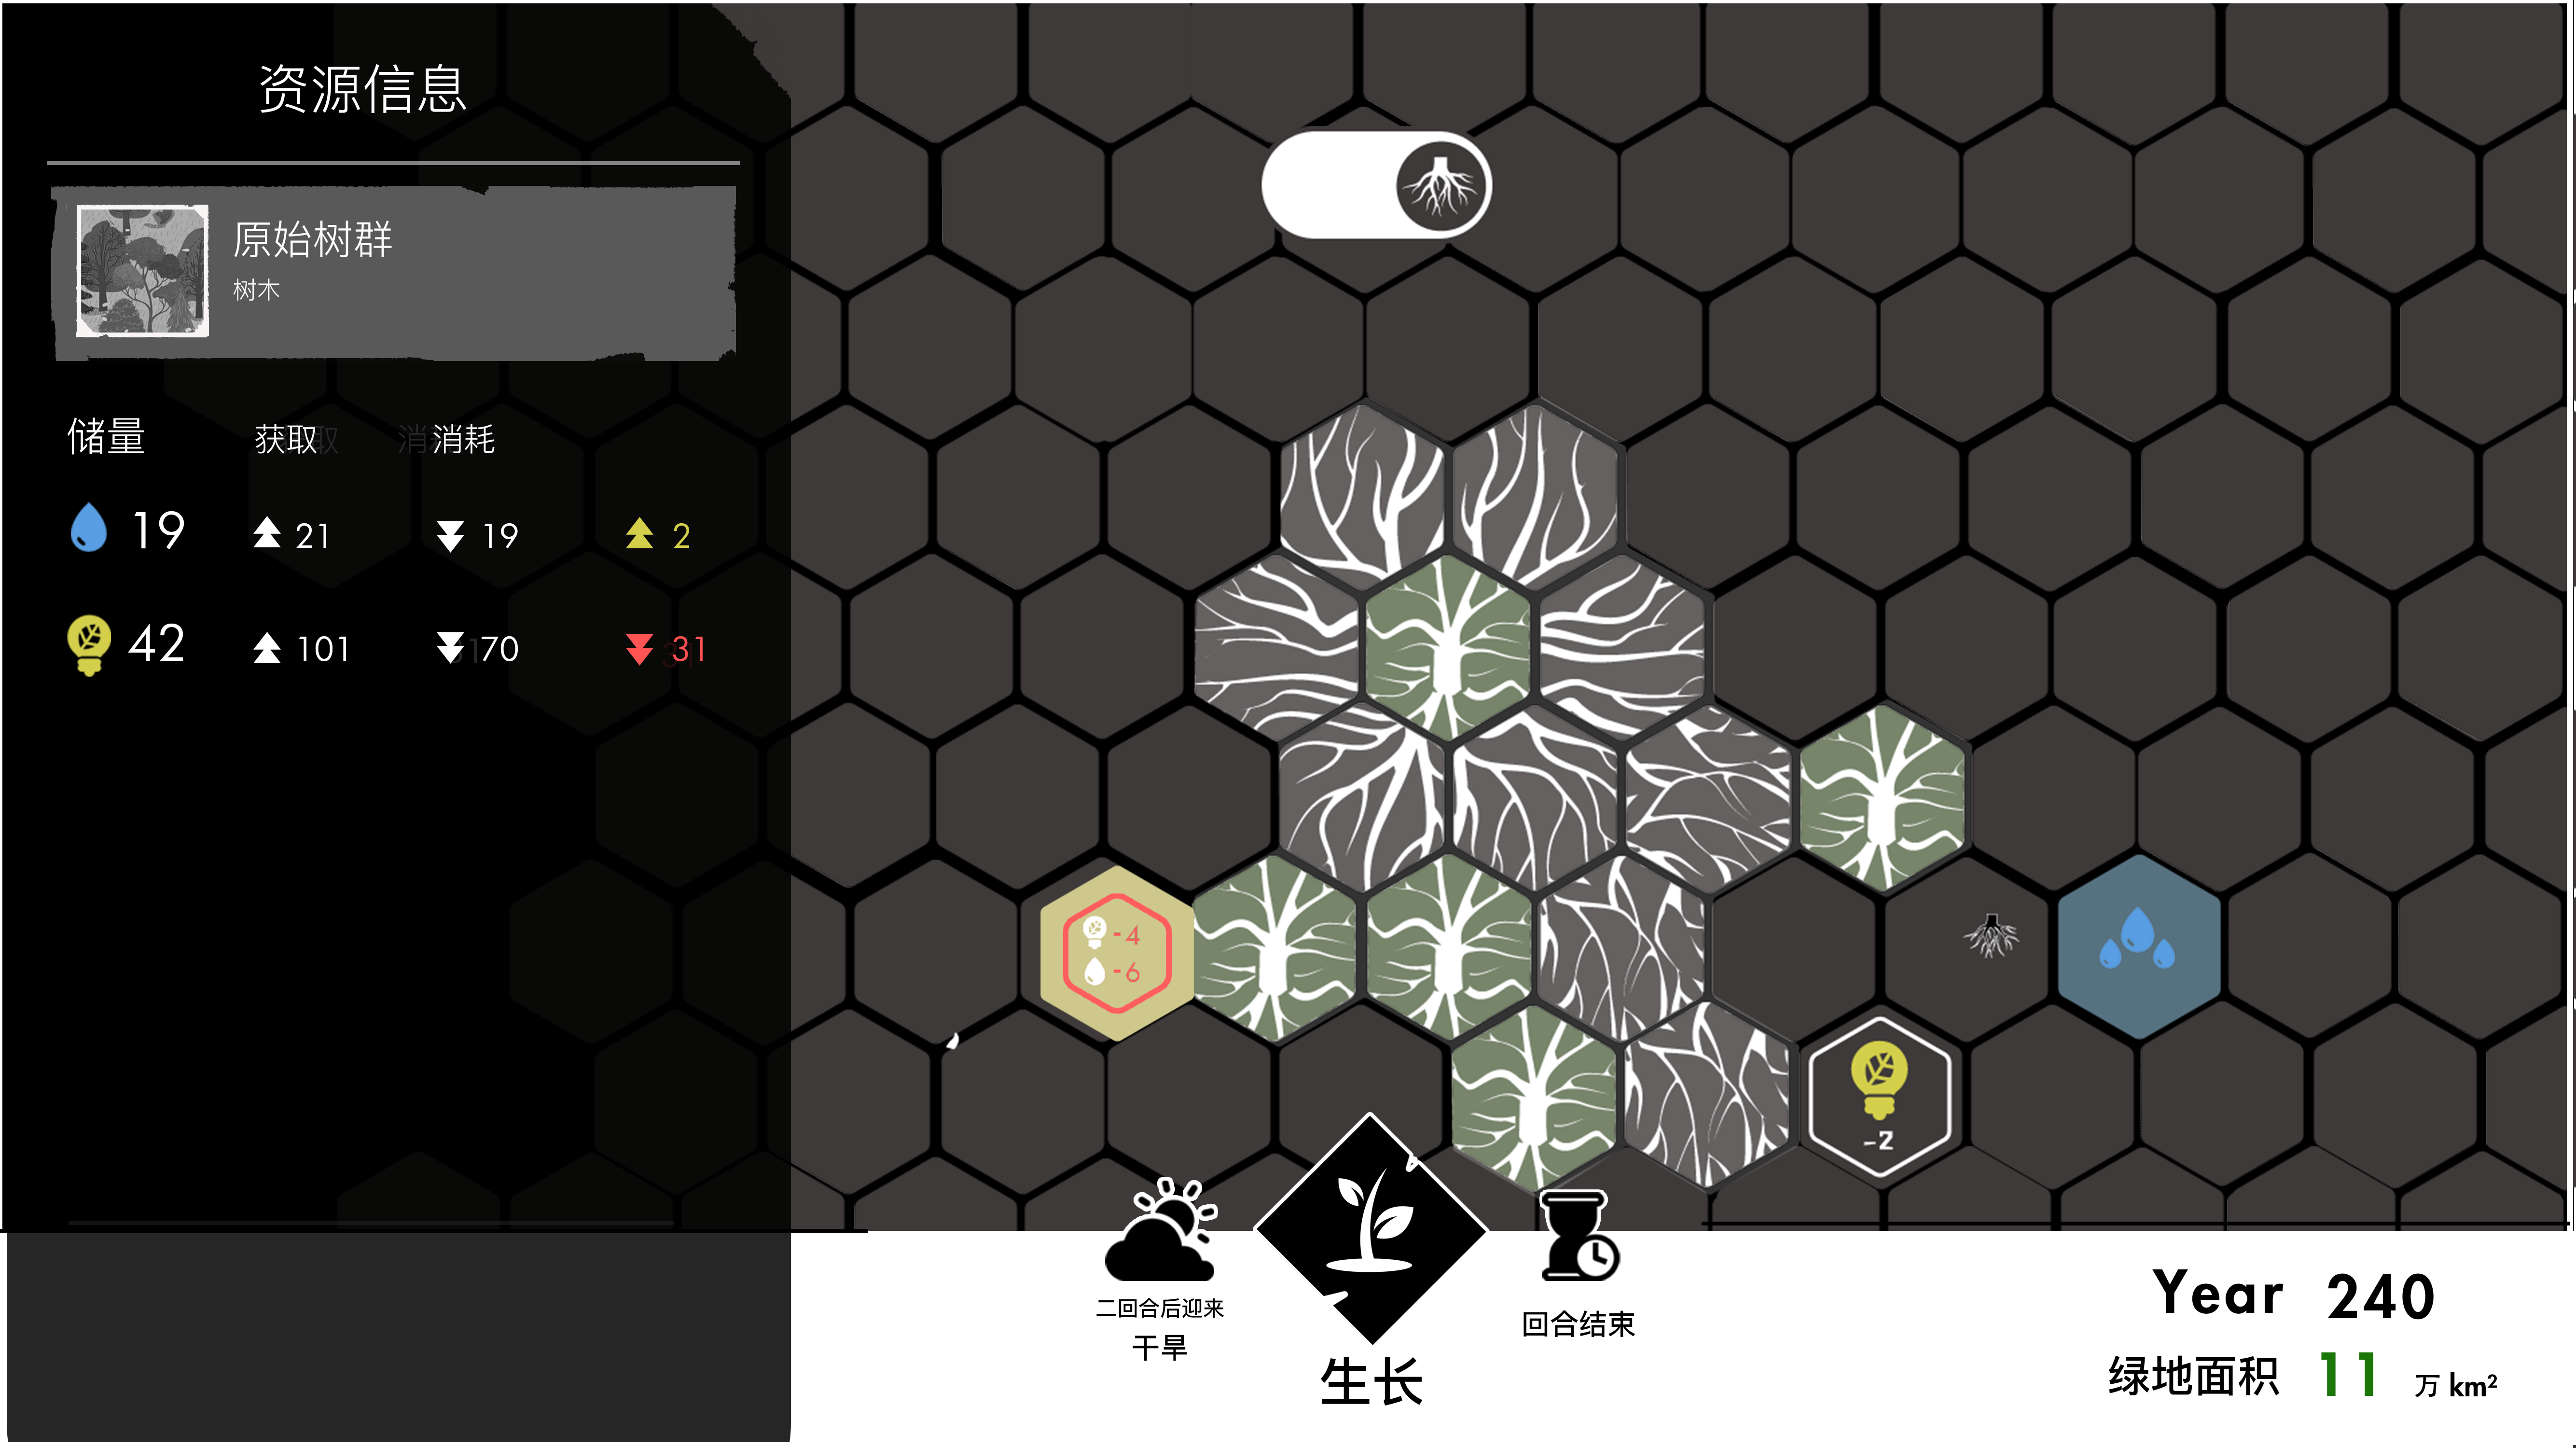
\includegraphics[width=0.8\textwidth]{Images/独木成林/dmzl2.png}
    \caption{独木成林\ 地下画面}
\end{figure}

\section{演示链接}
\begin{itemize}
    \item \textbf{试玩视频:}  \href{https://www.bilibili.com/video/BV18A41167H6/?vd_source=ead0ac501dfae814e19fd7d9f376d92d}{Bilibili视频}
    \item \textbf{Demo下载:}  \href{https://scyq.itch.io/oasis}{itch.io界面} 
    \item \textbf{GGJ2023参赛页面} \href{https://www.gmhub.com/game/2379}{GmHub}
\end{itemize}